%-------------------------------------------------------------------------------
\section{Performance Results}
%-------------------------------------------------------------------------------
\label{sec:perf-results}

% How is the ASP based solver performing?

The \clingo{} solver performance given a logic program depends on a number of factors.
First, the number of facts in a specific concretization. Second, the configuration and
various optimization parameters passed to the solver.

The solving process consists of four stages: \emph{setup}, \emph{load}, \emph{ground},
and \emph{solve}. The first two are preliminary phases and the other two perform the
solve. Specifically, the setup phase generates the facts for the given spec,
whereas the load phase loads the main logic program (i.e., the rules of the
software model) as a resource into the solver. The grounding phase comes first. Once we
have a grounded program, we can run the last phase: the full solve in \clingo{}.
%
We instrumented the solver to measure each phase.

% 
\begin{figure*}[htb]

    \centering
    \subfloat[][Ground times]{
    \label{subfig:deps_quartz_load}
        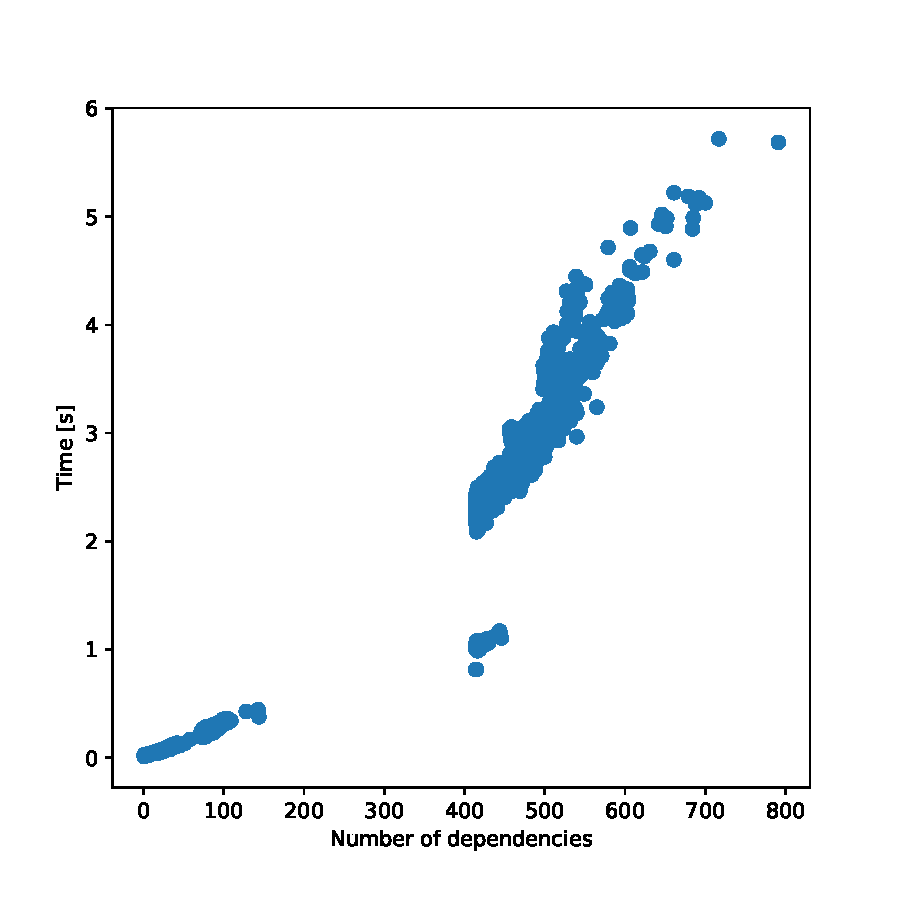
\includegraphics[width=0.32\textwidth]{figures/perf/deps_quartz_ground_fig.pdf}
    }\hfill%
    \subfloat[][Solve times]{
    \label{subfig:deps_quartz_solve}
        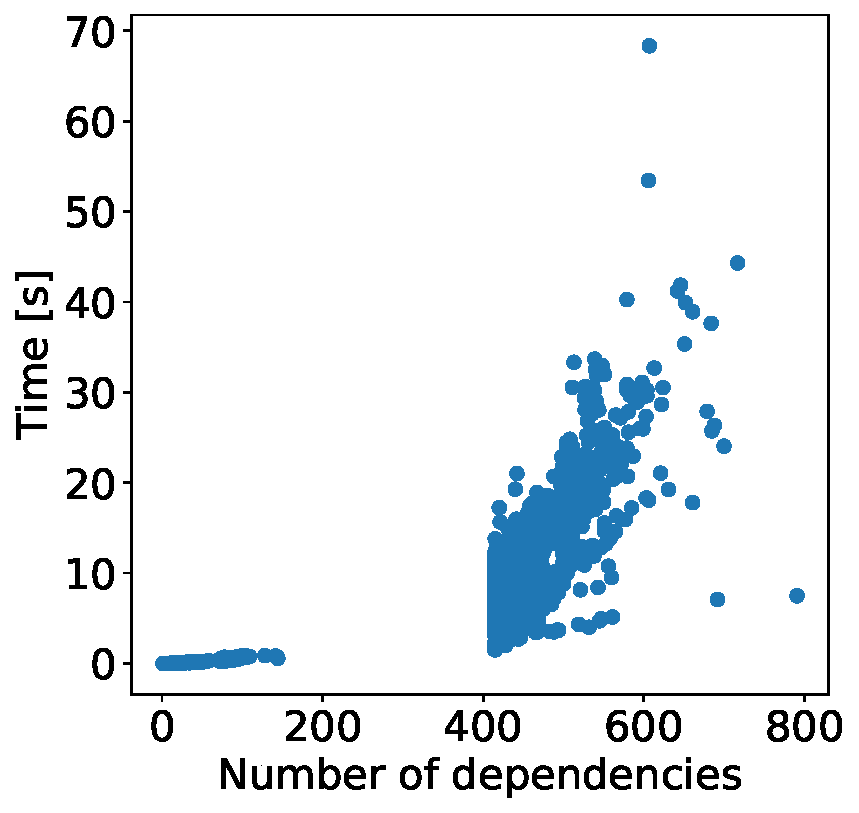
\includegraphics[width=0.32\textwidth]{figures/perf/deps_quartz_solve_fig.pdf}
    }\hfill%
    \subfloat[][Full solving times]{
    \label{subfig:deps_quartz_full}
        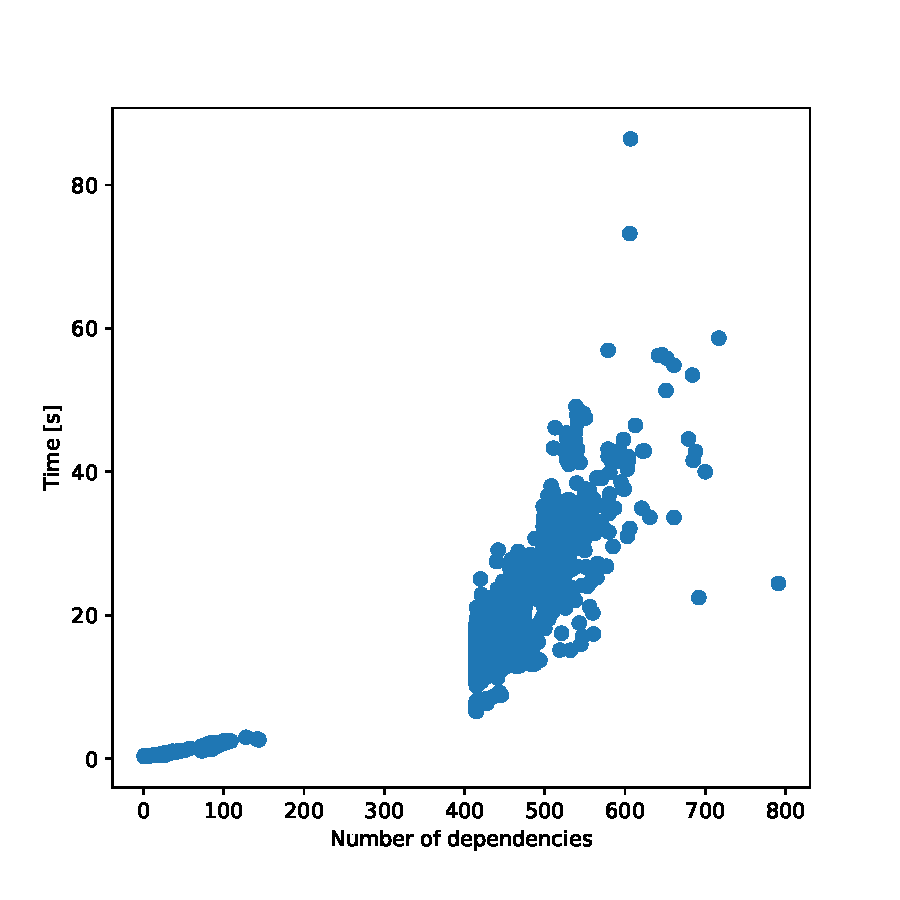
\includegraphics[width=0.32\textwidth]{figures/perf/deps_quartz_total_fig.pdf}
    }
    \caption{Solve times vs. number of dependent packages across all packages on the Quartz machine.}
    \label{fig:deps_quartz}

\end{figure*}


% 
\begin{figure*}[htb]

    \centering
    \subfloat[][Ground times]{
    \label{subfig:deps_lassen_load}
        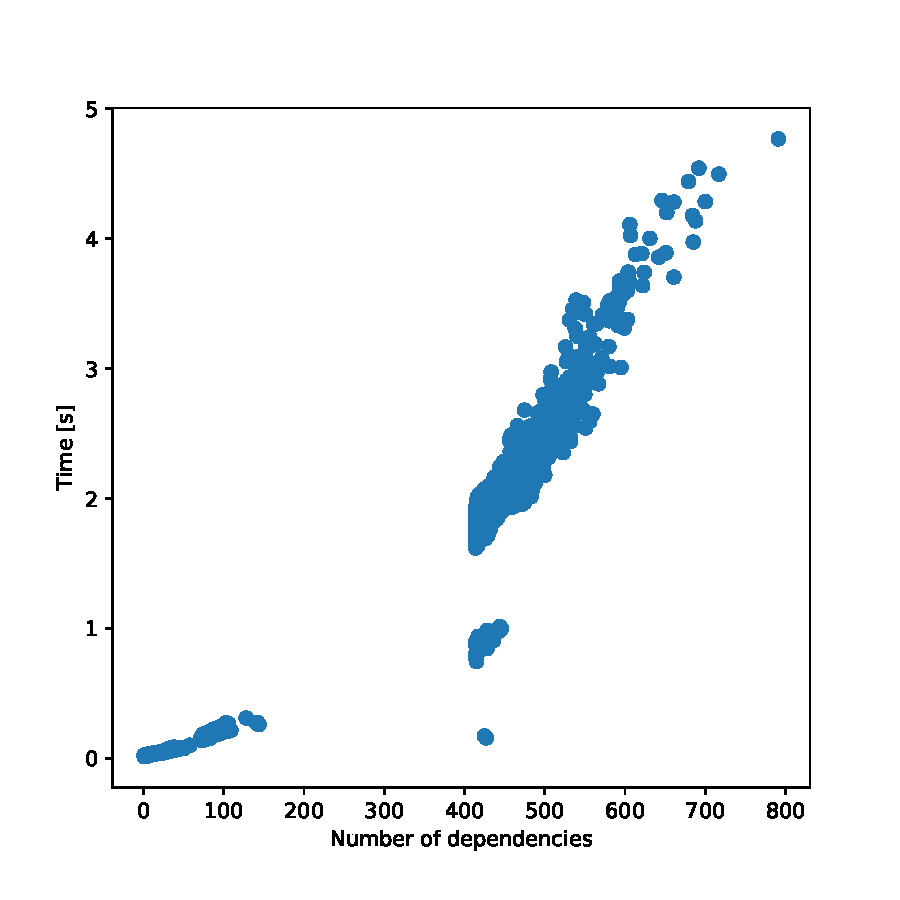
\includegraphics[width=\perfsubfigwidth\textwidth]{figures/perf/deps_lassen_ground_fig.pdf}
    }\hfill%
    \subfloat[][Solve times]{
    \label{subfig:deps_lassen_solve}
        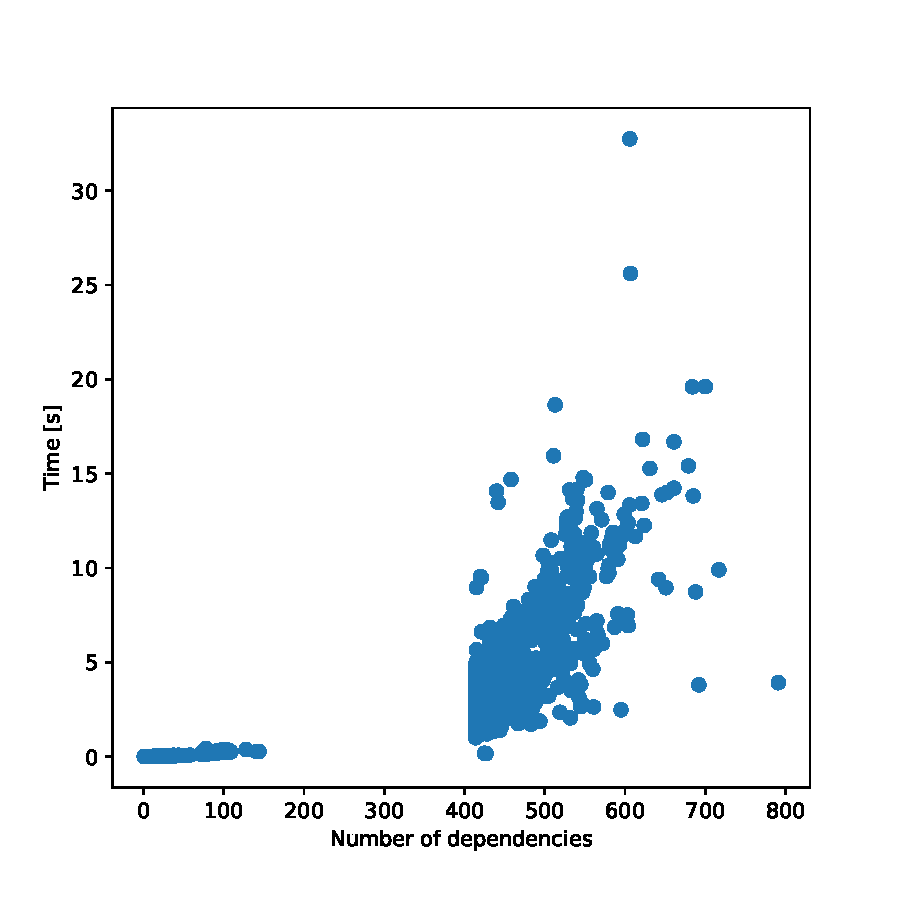
\includegraphics[width=\perfsubfigwidth\textwidth]{figures/perf/deps_lassen_solve_fig.pdf}
    }\hfill%
    \subfloat[][Full solving times]{
    \label{subfig:deps_lassen_full}
        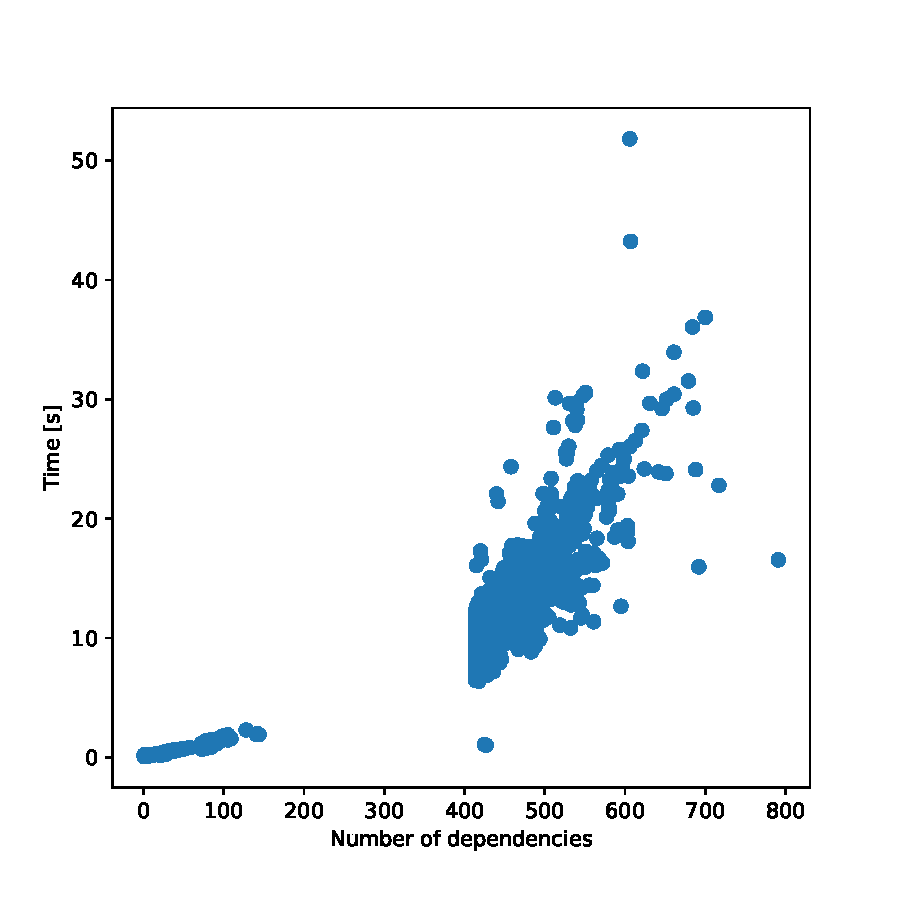
\includegraphics[width=\perfsubfigwidth\textwidth]{figures/perf/deps_lassen_total_fig.pdf}
    }
    \caption{Solve times vs. number of dependent packages across all packages on the Lassen machine.}
    \label{fig:deps_lassen}

\end{figure*}



\begin{figure*}[htb]

    \centering
    \subfloat[][Ground times vs. number of dependencies]{
    \label{subfig:deps_quartz_load_a}
        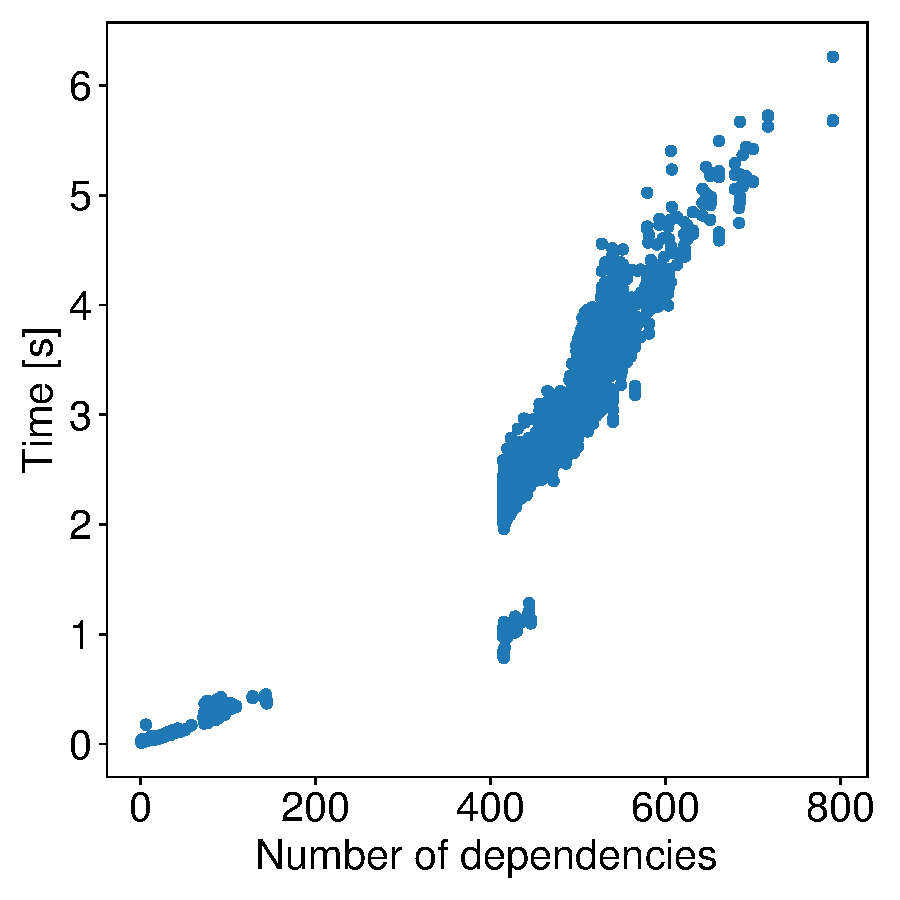
\includegraphics[width=\perfsubfigwidth\textwidth]{figures/new-quartz/deps_quartz_ground_fig.pdf}
    }\hfill%
    \subfloat[][Solve times vs. number of dependencies]{
    \label{subfig:deps_quartz_solve_a}
        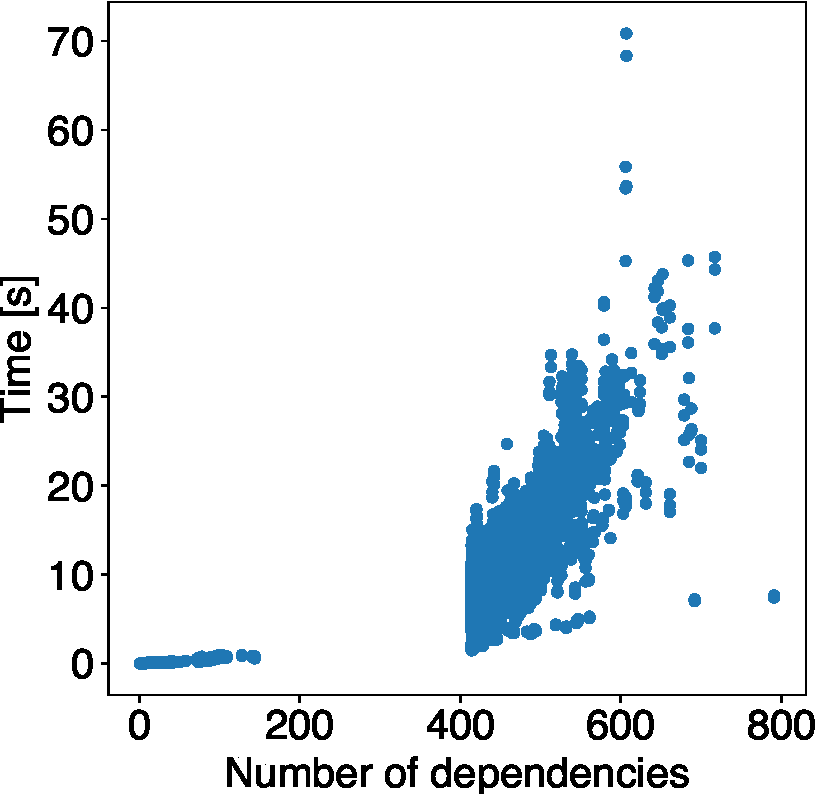
\includegraphics[width=\perfsubfigwidth\textwidth]{figures/new-quartz/deps_quartz_solve_fig.pdf}
    }\hfill%
    \subfloat[][Full solving times vs. number of dependencies]{
    \label{subfig:deps_quartz_full_a}
        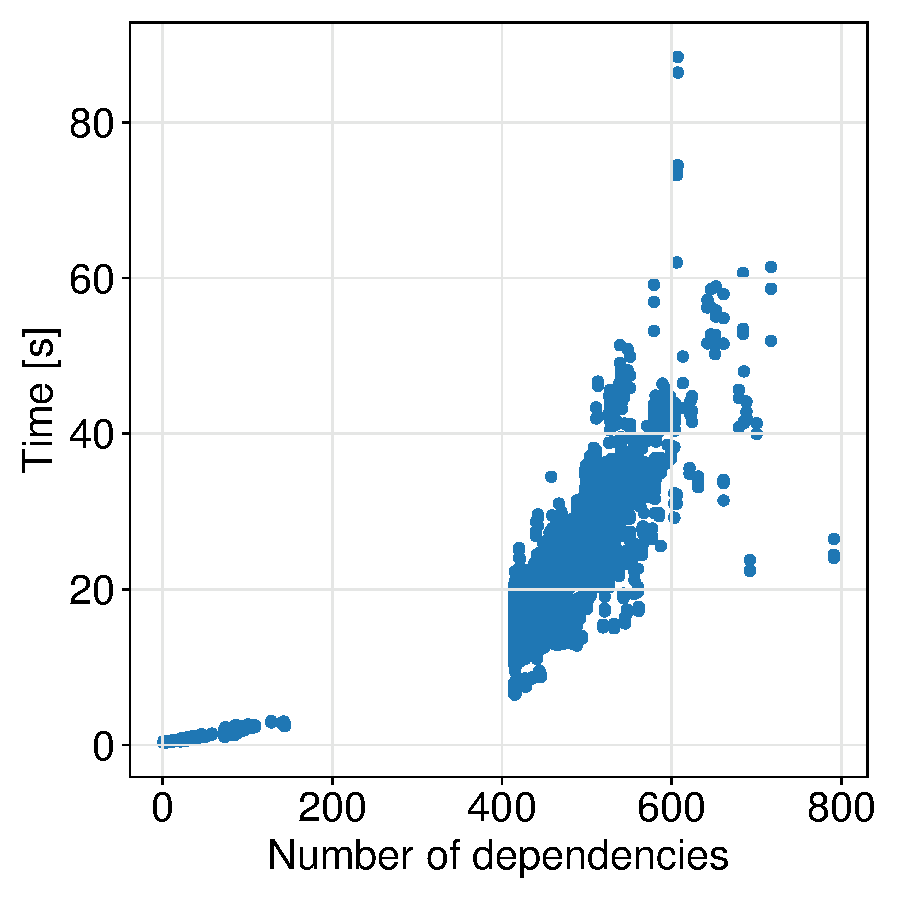
\includegraphics[width=\perfsubfigwidth\textwidth]{figures/new-quartz/deps_quartz_total_fig.pdf}
    }\hfill%
    \subfloat[][CDF of full solving times under various configurations]{
    \label{subfig:cdf_quartz_full_a}
        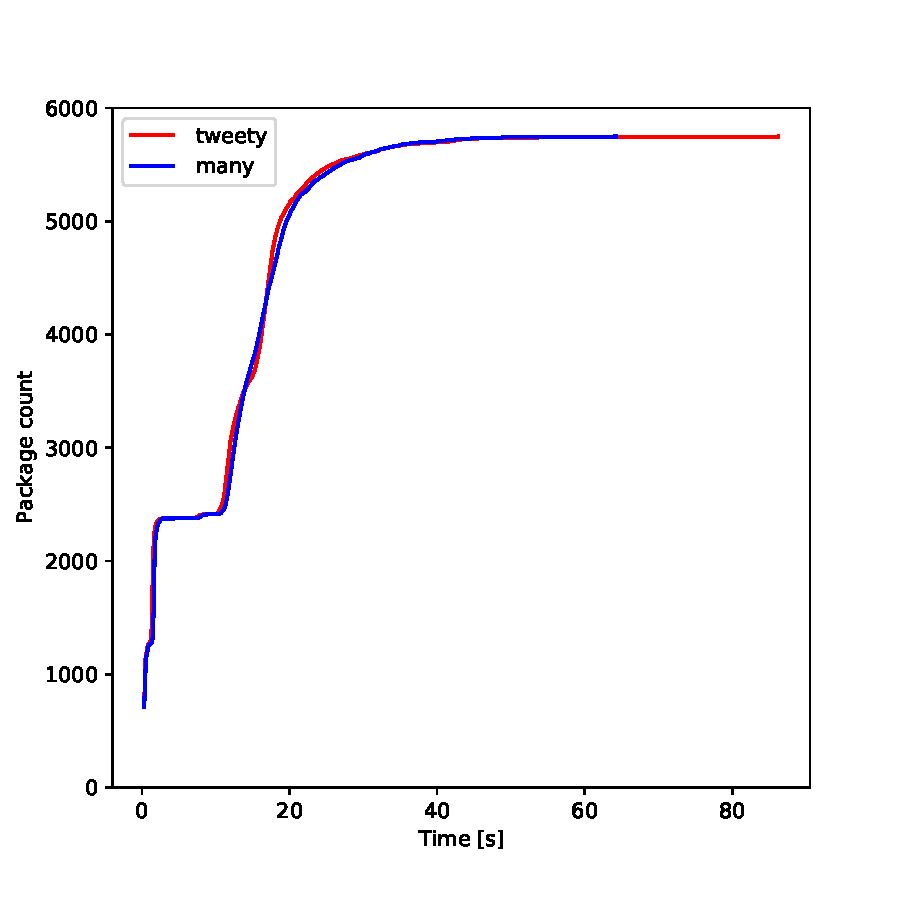
\includegraphics[width=\perfsubfigwidth\textwidth]{figures/perf/cdf_quartz_total_fig.pdf}
    }\\
    \subfloat[][CDF of setup times for different cache sizes across all E4S packages]{
    \label{subfig:cdf_e4s_quartz_load_a}
        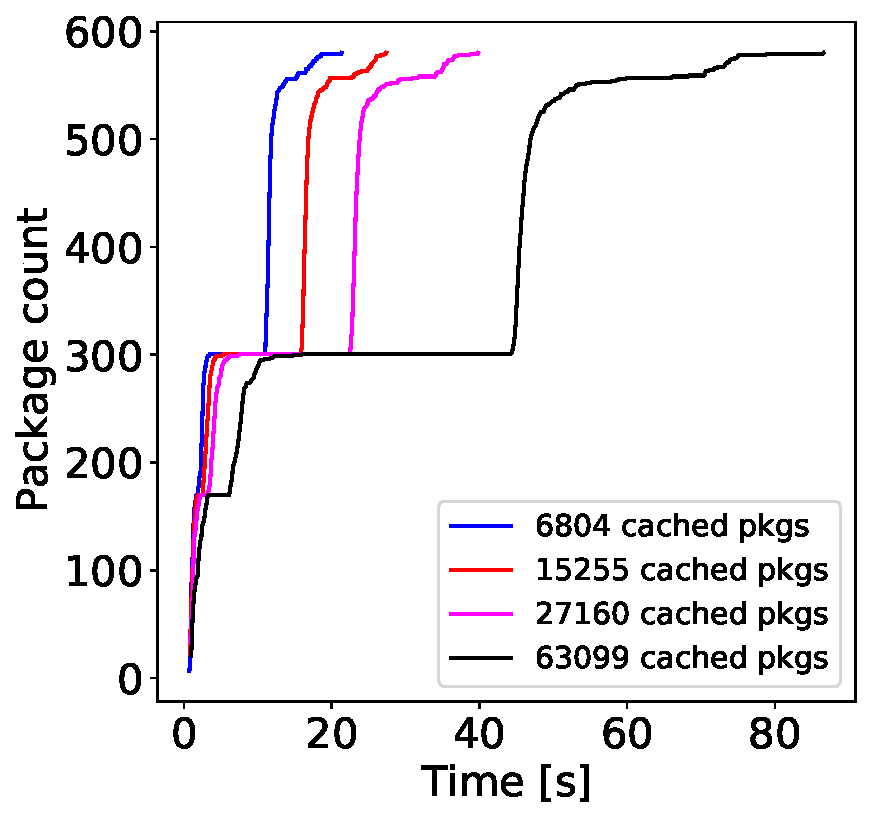
\includegraphics[width=\perfsubfigwidth\textwidth]{figures/perf/cdf_e4s_cache_quartz_setup_fig.pdf}
    }\hfill%
    \subfloat[][CDF of solve times for different cache sizes across all E4S packages]{
    \label{subfig:cdf_e4s_quartz_solve_a}
        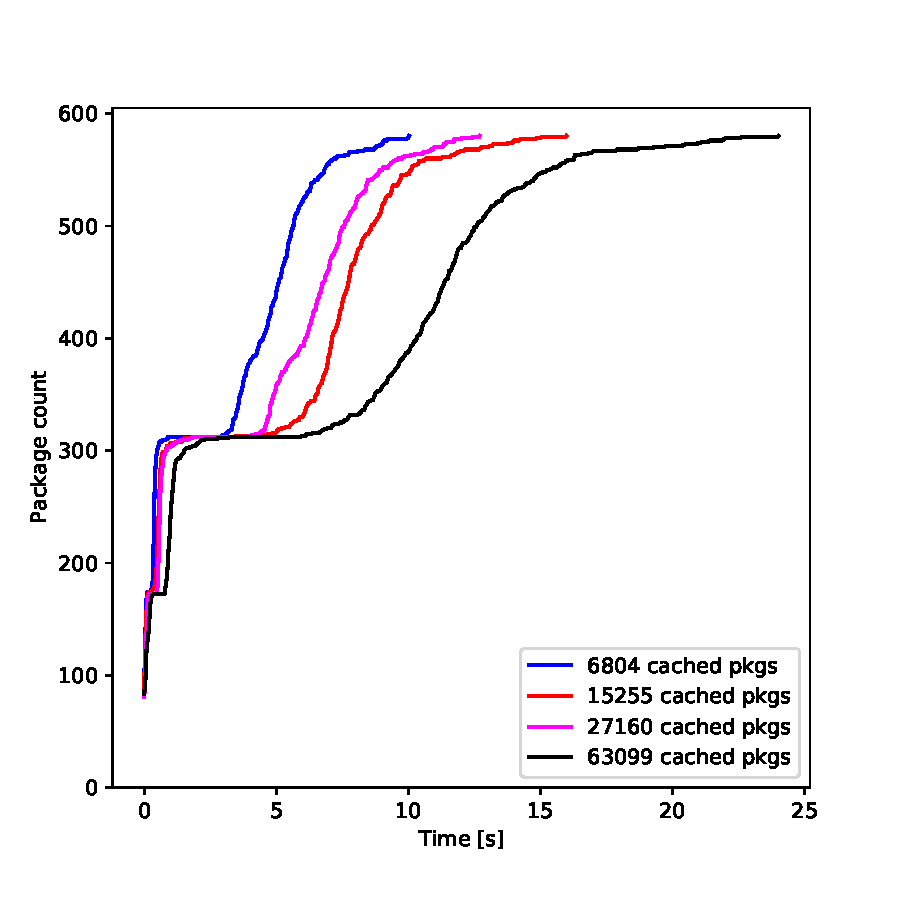
\includegraphics[width=\perfsubfigwidth\textwidth]{figures/perf/cdf_e4s_cache_quartz_solve_fig.pdf}
    }\hfill%
    \subfloat[][CDF of total solver times for different cache sizes across all E4S packages]{
    \label{subfig:cdf_e4s_quartz_full_a}
        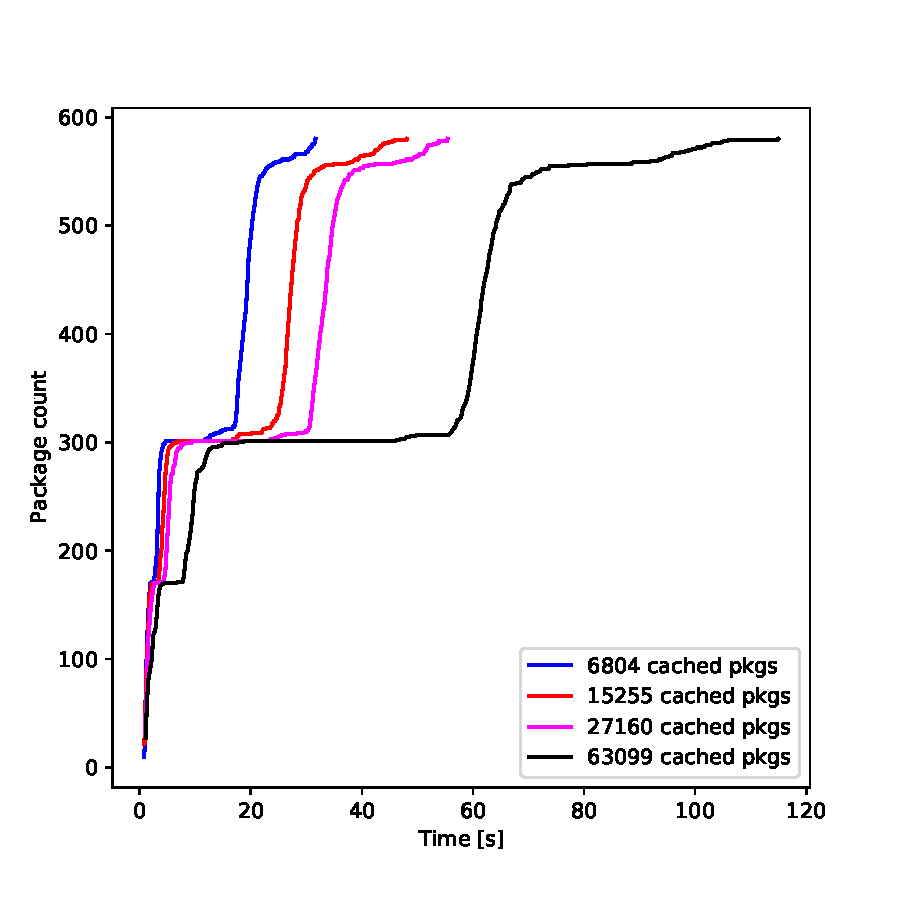
\includegraphics[width=\perfsubfigwidth\textwidth]{figures/perf/cdf_e4s_cache_quartz_total_fig.pdf}
    }\hfill%
    \subfloat[][CDF of old concretizer concretization times and \clingo{} total solve times]{
    \label{subfig:cdf_old_vs_new_a}
        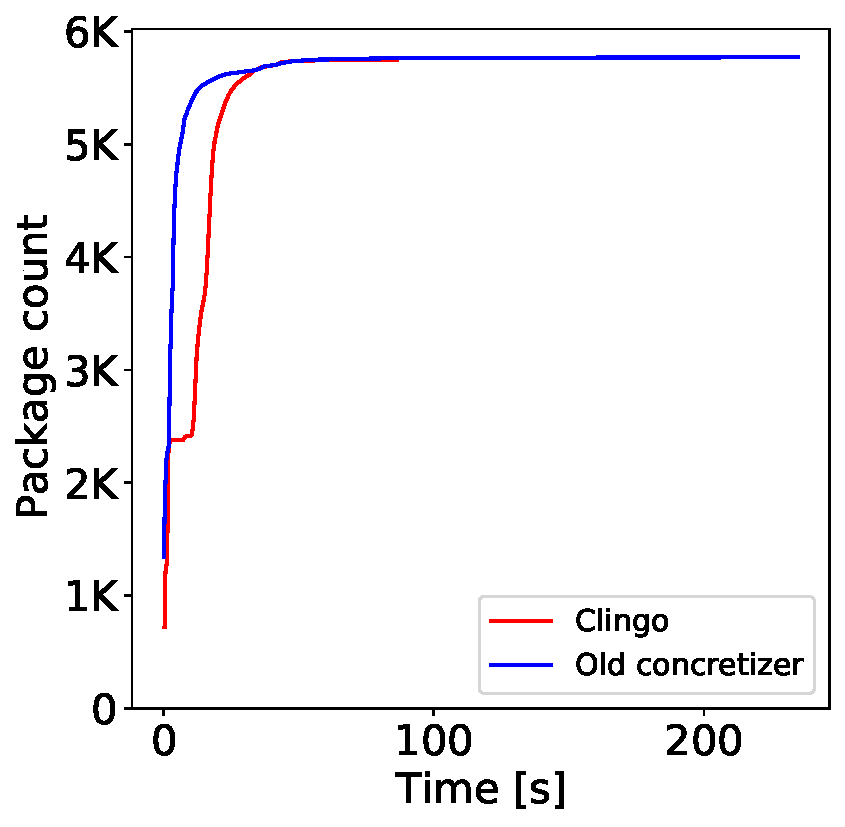
\includegraphics[width=\perfsubfigwidth\textwidth]{figures/perf/cdf_quartz_old_vs_clingo.pdf}
    }

    \caption{Performance figures of solving times across all packages on Quartz.\vspace{-1em}}
    \label{fig:all_perf}

\end{figure*}


\subsection{System Setup}

All performance runs were executed on a single node each of the Quartz and Lassen
supercomputers at [institution].
%at Lawrence Livermore National Laboratory (LLNL)~\cite{llnl:hpc}.
Quartz is an Intel-based 3.3 PF machine, where each node comprises two Intel Xeon
E5-2695 v4 (Haswell) processors and 128GB of memory. The Lassen machine is a smaller
variant of Sierra, a 125 PF capability supercomputer at LLNL. Each node on Lassen has
two IBM Power9 little-endian processors and four NVIDIA Tesla V100 (Volta) GPUs. There
are 256GB of memory on each node. No hardware accelerators were used in any of our
testing. Experiments ran with NFSv3.

\subsection{Solve timings for all packages}

In this section we examine the solving times for all the packages. First, we focus on the relation between the solving times and the number of dependencies for each package.

For number of dependencies, we measured the number of possible
dependencies added to the solve, rather than the total dependencies in
the result, because it is a closer measure of the necessary work for
the solver. This leads to natural clustering in the number of
dependencies, as many simple dependencies lead to large numbers of
potential dependencies that dwarf other differences between specs.

Figures~\ref{subfig:deps_quartz_load_a}, \ref{subfig:deps_quartz_solve_a}, and ~\ref{subfig:deps_quartz_full_a} show the grounding, solve, and full solving (i.e., involving all the stages) times for all the packages on Quartz. The results on Lassen are comparable to Quartz and are omitted to save space. Load times, as one would expect, were not affected by the number of packages. Also, the setup times are the same order of magnitude as ground times and do not depend on \clingo{}'s performance so they were omitted in favor of showing times that are directly dependent on \clingo{}. We used the \clingo{}'s "tweety" configuration and "usc,one" optimization strategy for running the solving process. Further below we explore the differences in solving times between these different strategies.

We can see from the figures that the time increases as the number of possible package dependencies increases. This is because increased number of possible dependencies leads to a larger number of facts and a bigger logic program overall. We measure possible dependencies rather than actual dependencies of the result because possible dependencies better measure the size of the problem space. In particular, when many packages can provide a virtual dependency like the Message Passing Interface (MPI), much of the potential solve space is not present in the final result when a single MPI implementation is chosen.

Figure~\ref{subfig:deps_quartz_full_a} also shows that there are two major clusters in the execution times. The clusters are separated by a gap in the possible dependencies. One cluster contains packages with less than 200 possible dependencies, whereas, the other major cluster contains packages with more than 400 possible dependencies. This natural clustering occurs because some low-level dependencies have options that can trigger huge potential dependency trees, and the gap is between packages that can include those dependencies and those that cannot. For example, any package that can depend on MPI in any possible configuration of it and its dependencies involves at least 452 possible dependencies. Since many unusual but technically valid package configurations can create circular dependencies between MPI and build tools (e.g. \texttt{mpilander} provides MPI and \texttt{mpilander -> cmake -> qt -> valgrind -> mpi}), in practice a gap forms between the packages that (mostly) all can depend on MPI, and those that cannot. While the solver excludes the configurations that actually produce circular dependencies, these cycles expand the solution space of the solver and therefore affect performance.

% TODO: Can we confirm this?? My explanation above is slightly vague -- GBB
% The gap occurs because of dependency on \emph{cmake}, which itself depends cumulatively on more than 400 packages.

% 
\begin{figure*}[htb]

    \centering
    \subfloat[][Ground times]{
    \label{subfig:cdf_quartz_ground}
        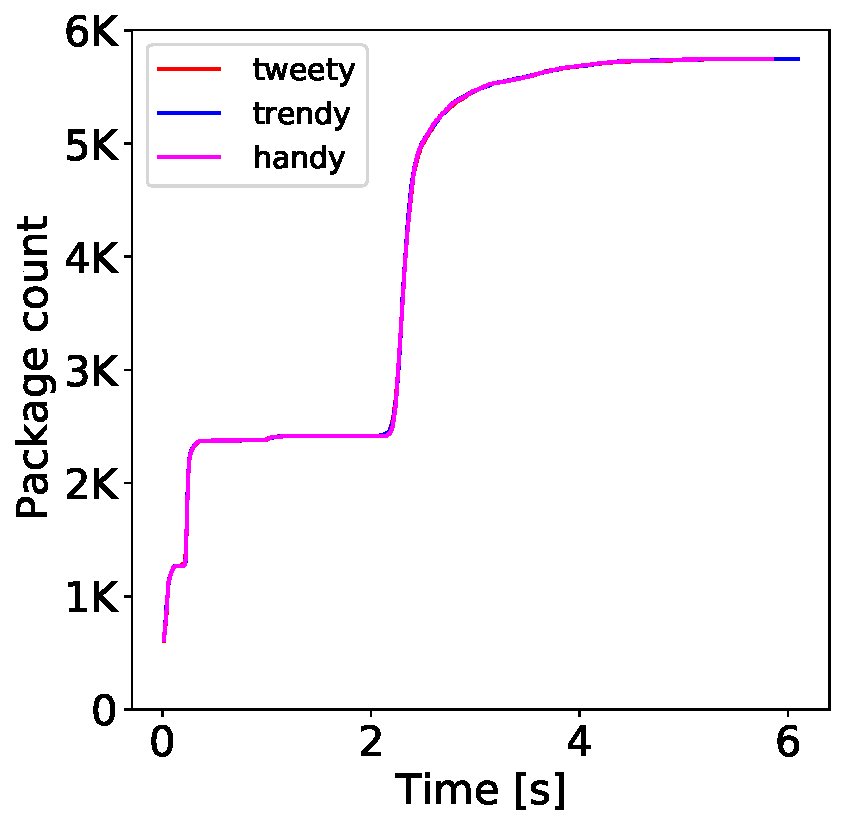
\includegraphics[width=\perfsubfigwidth\textwidth]{figures/perf/cdf_quartz_ground_fig.pdf}
    }\hfill%
    \subfloat[][Solve times]{
    \label{subfig:cdf_quartz_solve}
        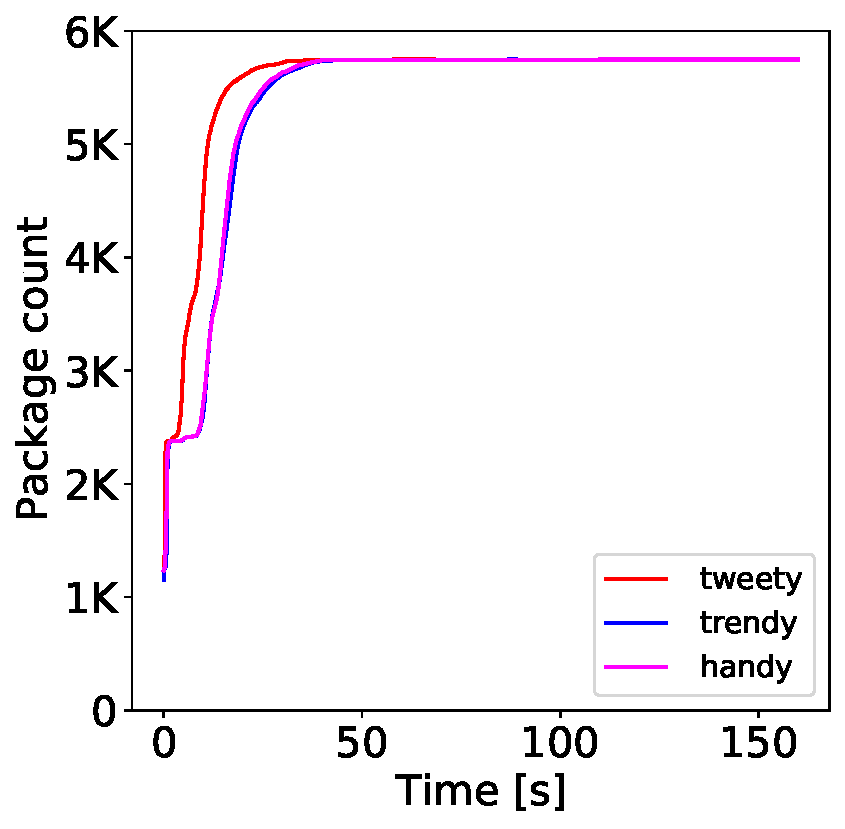
\includegraphics[width=\perfsubfigwidth\textwidth]{figures/perf/cdf_quartz_solve_fig.pdf}
    }\hfill%
    \subfloat[][Full solving times]{
    \label{subfig:cdf_quartz_full}
        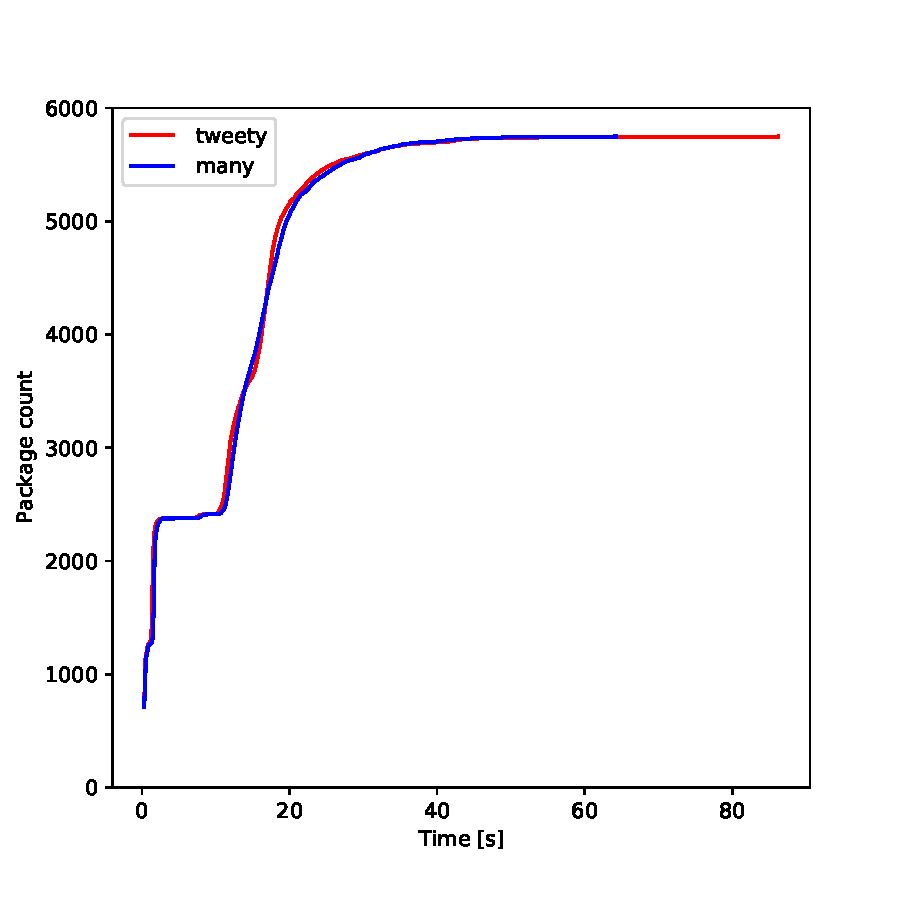
\includegraphics[width=\perfsubfigwidth\textwidth]{figures/perf/cdf_quartz_total_fig.pdf}
    }
    \caption{Cumulative distribution of solve times across all packages on the Quartz machine.}
    \label{fig:cdf_quartz}

\end{figure*}


% 
\begin{figure}[htb]

    \centering
    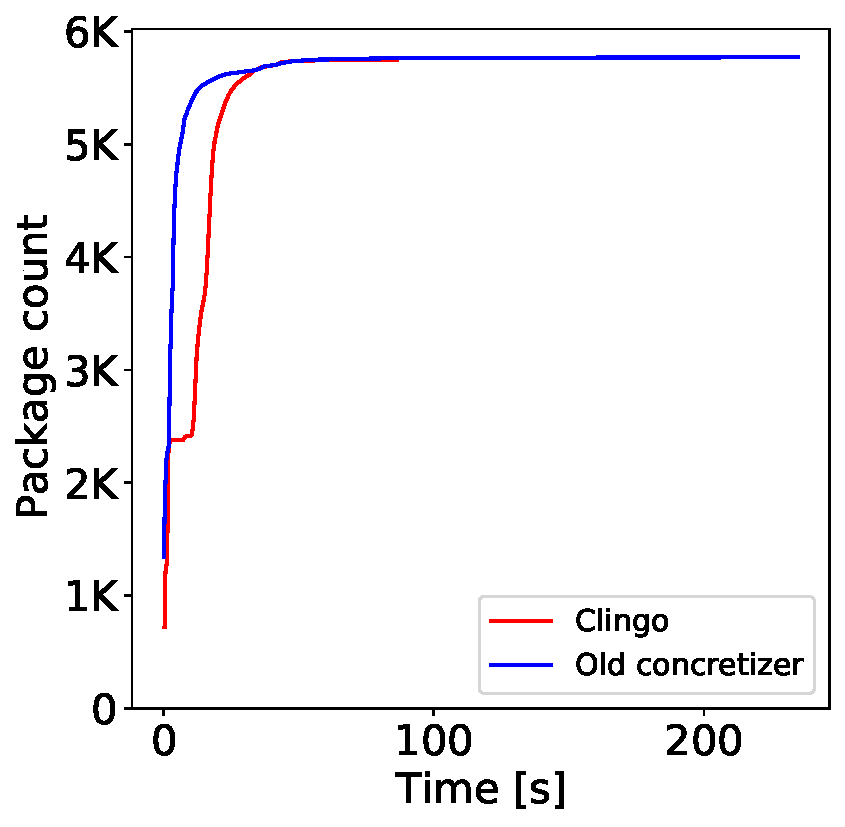
\includegraphics[width=0.3\textwidth]{figures/perf/cdf_quartz_old_vs_clingo.pdf}
    \caption{Cumulative distribution of old concretizer concretization times and \clingo{} solve times across all packages on Quartz.}
    \label{fig:cdf_quartz_old_vs_new}

\end{figure}


% 
\begin{figure*}[htb]

    \centering
    \subfloat[][Load times]{
    \label{subfig:cdf_lassen_load}
        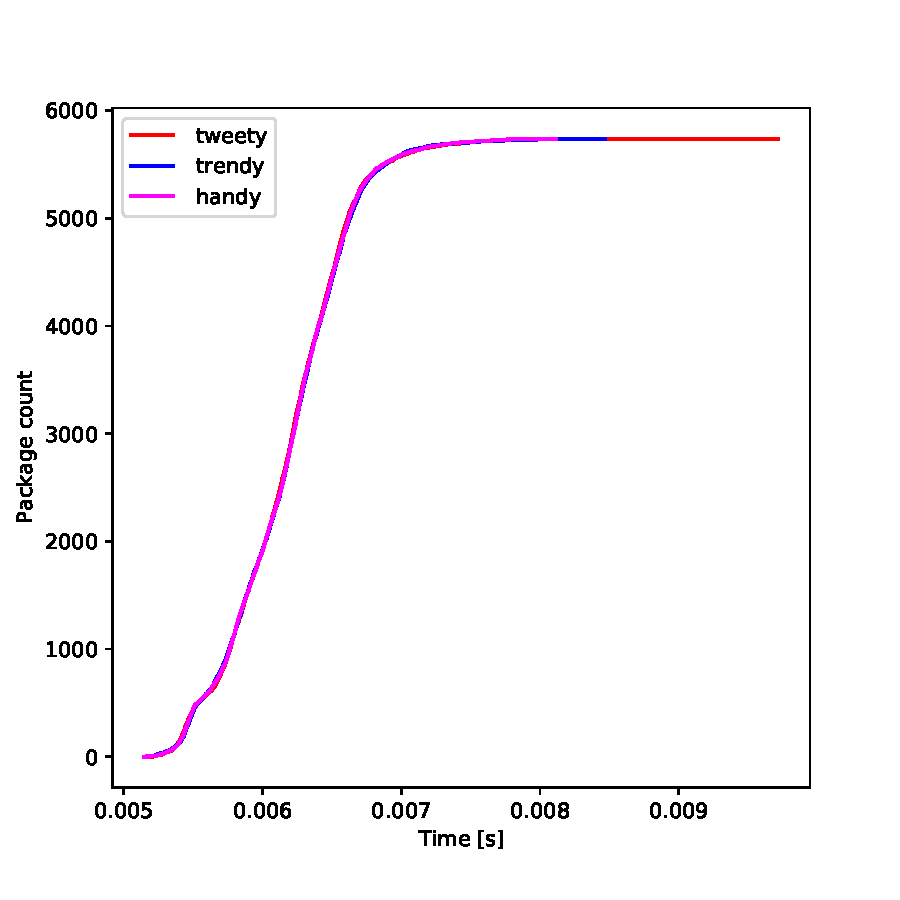
\includegraphics[width=0.32\textwidth]{figures/perf/cdf_lassen_load_fig.pdf}
    }\hfill%
    \subfloat[][Solve times]{
    \label{subfig:cdf_lassen_solve}
        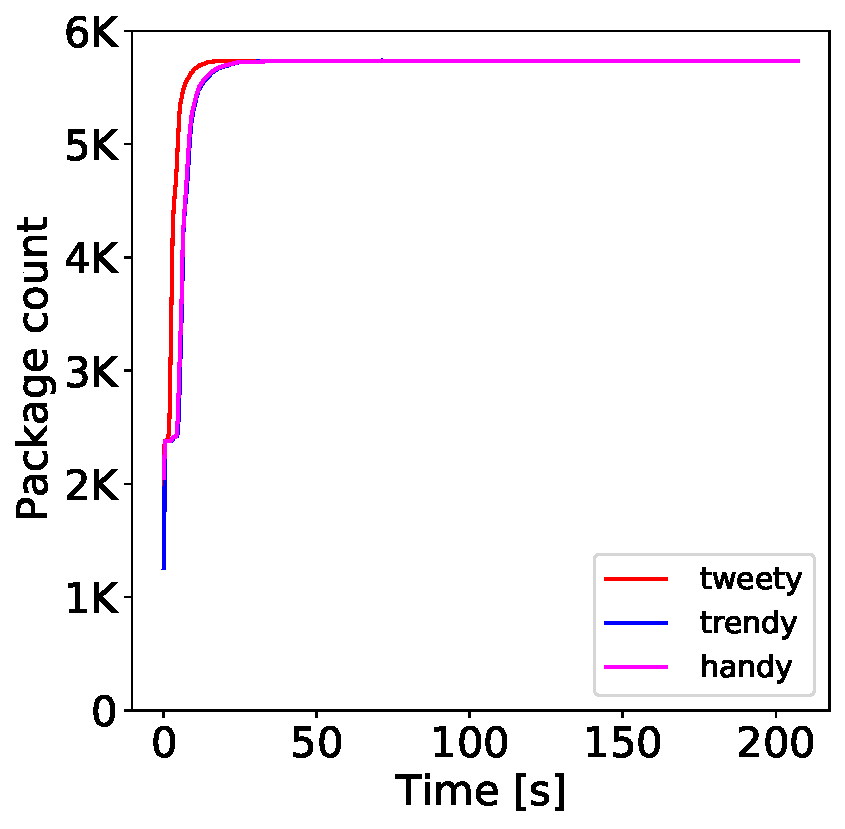
\includegraphics[width=0.32\textwidth]{figures/perf/cdf_lassen_solve_fig.pdf}
    }\hfill%
    \subfloat[][Full solving times]{
    \label{subfig:cdf_lassen_full}
        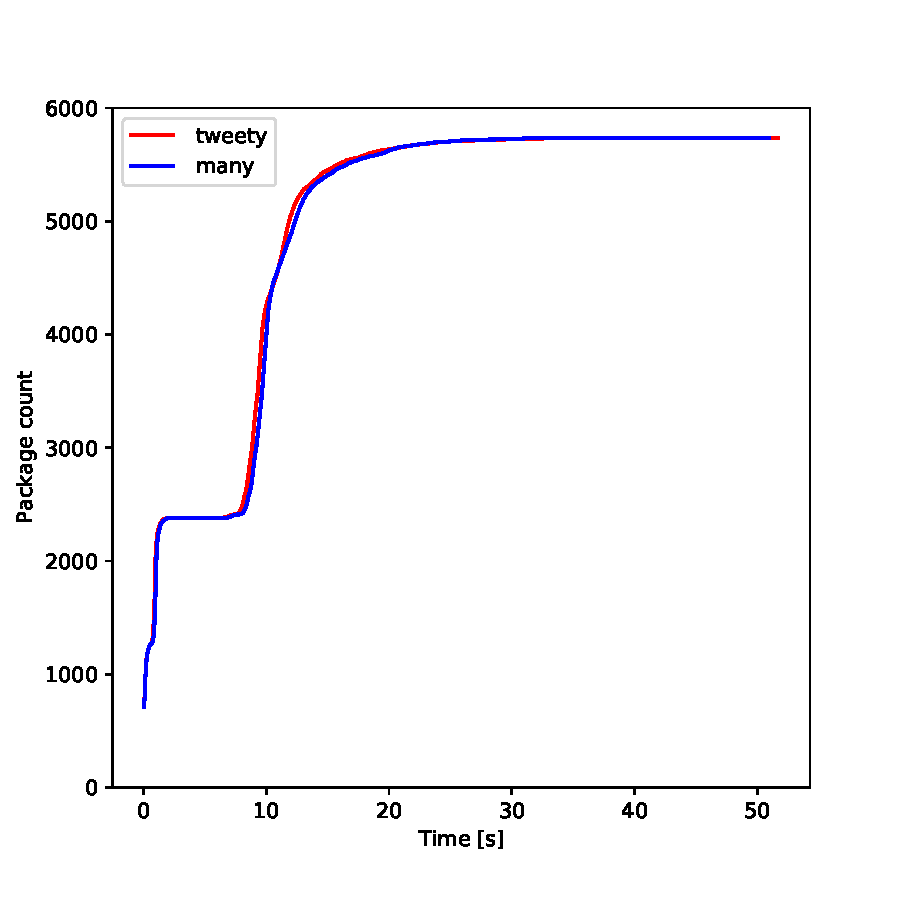
\includegraphics[width=0.32\textwidth]{figures/perf/cdf_lassen_total_fig.pdf}
    }
    \caption{Cumulative distribution of solve times across all packages on the Lassen machine.}
    \label{fig:cdf_quartz}

\end{figure*}


Besides dependencies another set of factors that influences the execution times are \clingo{} parameters. Specifically, \clingo{} defines six configuration presets: \emph{frumpy}, \emph{jumpy}, \emph{tweety}, \emph{trendy}, \emph{crafty}, and \emph{handy}. Each preset sets numerous low level parameters that control different aspects of the solver. In our performance study, we specifically focus on three configurations: \emph{tweety} -- geared towards typical ASP programs, \emph{trendy} -- geared towards industrial problems, and \emph{handy} -- geared towards large problems.

%Figures~\ref{subfig:cdf_quartz_ground_a}, \ref{subfig:cdf_quartz_solve_a}, and~\ref{subfig:cdf_quartz_full_a} show the cumulative distribution of the solve times under \emph{tweety}, \emph{trendy}, and \emph{handy} configurations on Quartz.
Figure~\ref{subfig:cdf_quartz_full_a} shows the cumulative distribution of full solve times  \emph{tweety}, \emph{trendy}, and \emph{handy} configurations on Quartz.
The results on Lassen are comparable to Quartz and are omitted to save space. The vast majority of packages are fully solved in under 25 seconds on both machines. We also saw (figure omitted) that there is no difference in ground times between the different configurations. This suggests that most low level parameters that are tweaked by each configuration control the actual solving phase. The figures clearly indicate that \emph{tweety} performs better than the other configurations we benchmarked. This is, therefore, the default configuration used in the concretization process.

Figure~\ref{subfig:cdf_old_vs_new_a} shows the the cumulative distribution of the old concretizer concretization times and \clingo{} total solve times (under \emph{tweety} configuration) on Quartz. Figure~\ref{subfig:deps_quartz_full_a} shows us that about 2.2K packages belong to the cluster with less than 200 dependencies, which means that the dependency trees of these packages are smaller. This leads to shorter ground and solve times and that makes \clingo{}'s times correspond to old concretizer times for these packages. The packages in the other cluster have potentially huge dependency trees that increase the total solving times and that is reflected in the deviation of \clingo{}'s times in Figure~\ref{subfig:cdf_old_vs_new_a} from the old concretizer times.

% - other properties?
% - --single-shot vs. no single-shot?
% - different tactics?

\subsection{Solve timings for all packages with reuse}

In this subsection, we examine the performance of the solver with the \emph{reuse} flag switched on. As described in Section~\ref{sec:reuse}, reusing packages in a buildcache increases the number of facts proportionally to the number of cached packages.

% 
\begin{figure*}[htb]

    \centering
    \subfloat[][Setup times]{
    \label{subfig:cdf_e4s_quartz_load}
        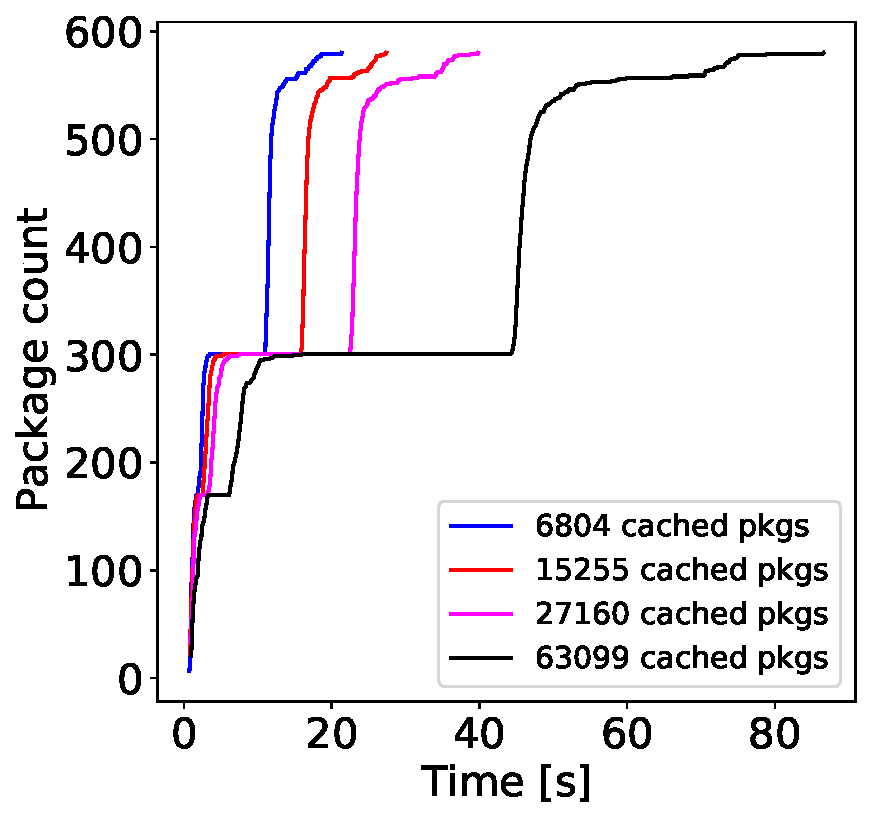
\includegraphics[width=\perfsubfigwidth\textwidth]{figures/perf/cdf_e4s_cache_quartz_setup_fig.pdf}
    }\hfill%
    \subfloat[][Solve times]{
    \label{subfig:cdf_e4s_quartz_solve}
        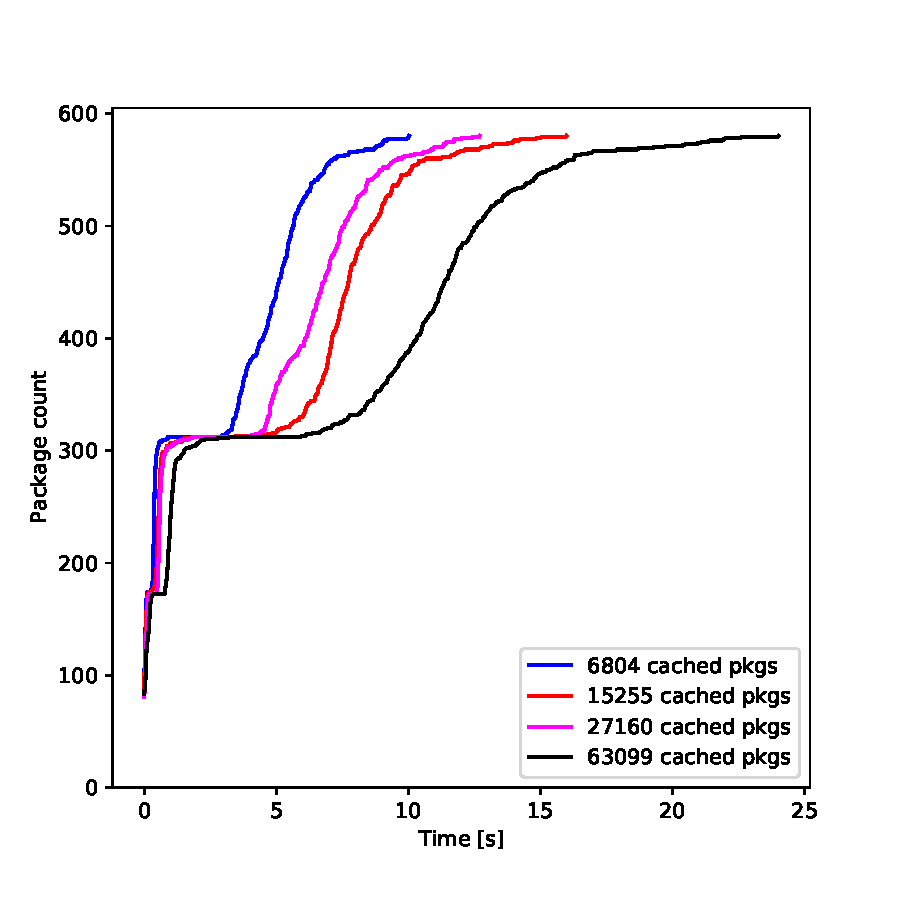
\includegraphics[width=\perfsubfigwidth\textwidth]{figures/perf/cdf_e4s_cache_quartz_solve_fig.pdf}
    }\hfill%
    \subfloat[][Total solver times]{
    \label{subfig:cdf_e4s_quartz_full}
        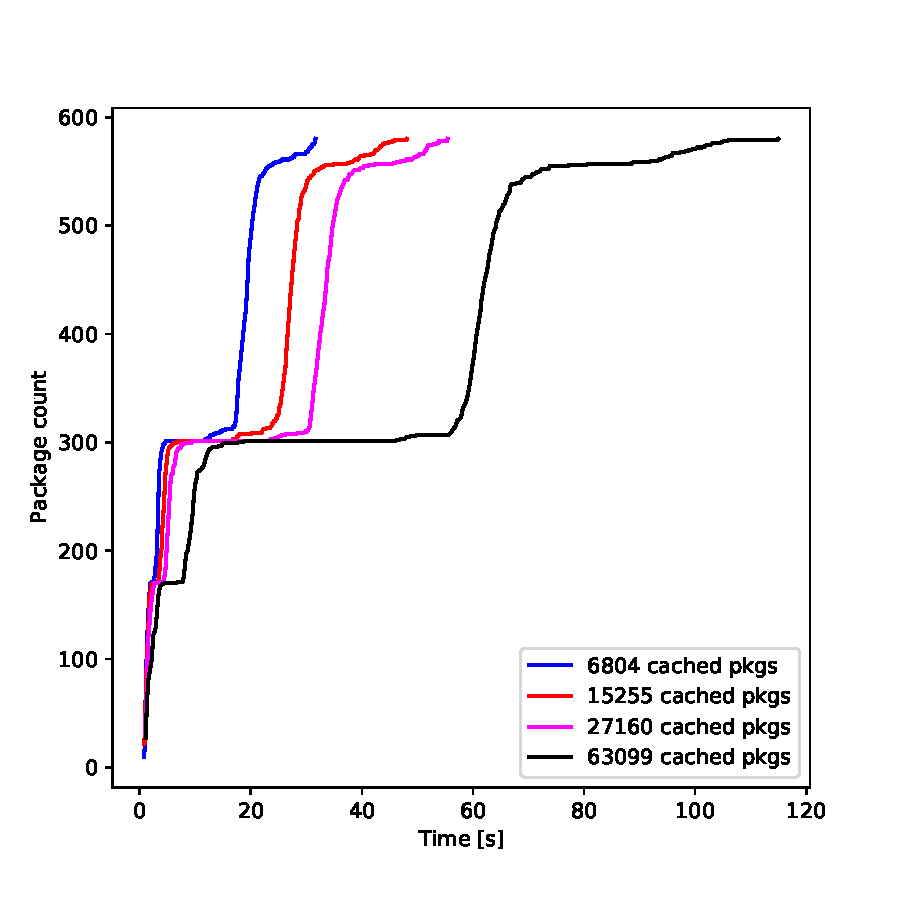
\includegraphics[width=\perfsubfigwidth\textwidth]{figures/perf/cdf_e4s_cache_quartz_total_fig.pdf}
    }
    \caption{Cumulative distribution of solve times for different cache sizes across all E4S packages on the Quartz machine.}
    \label{fig:cdf_e4s_quartz}

\end{figure*}


% 
\begin{figure*}[htb]

    \centering
    \subfloat[][Setup times]{
    \label{subfig:cdf_e4s_lassen_load}
        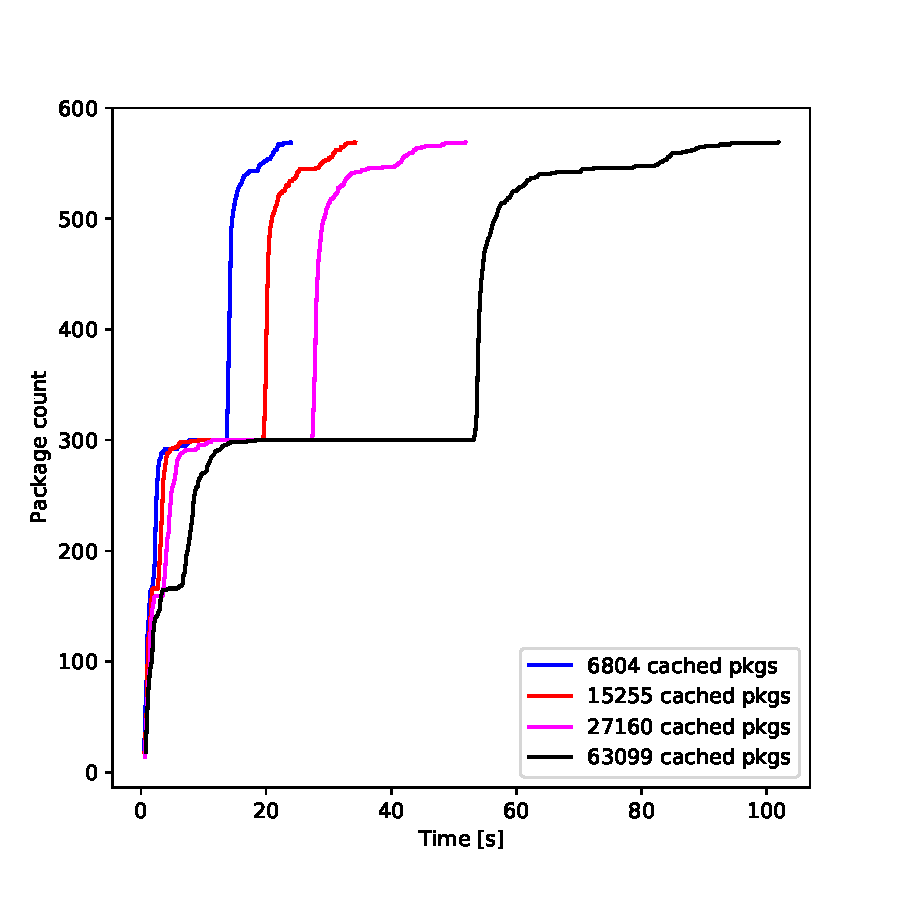
\includegraphics[width=0.32\textwidth]{figures/perf/cdf_e4s_cache_lassen_setup_fig.pdf}
    }\hfill%
    \subfloat[][Solve times]{
    \label{subfig:cdf_e4s_lassen_solve}
        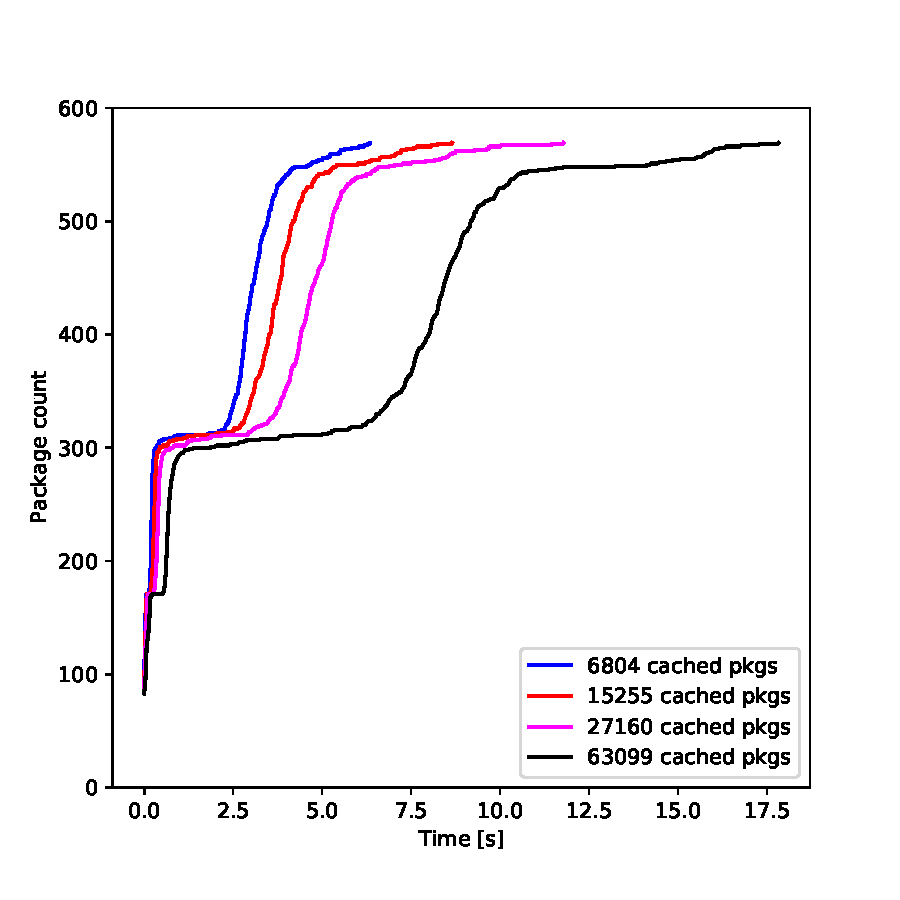
\includegraphics[width=0.32\textwidth]{figures/perf/cdf_e4s_cache_lassen_solve_fig.pdf}
    }\hfill%
    \subfloat[][Total solver times]{
    \label{subfig:cdf_e4s_lassen_full}
        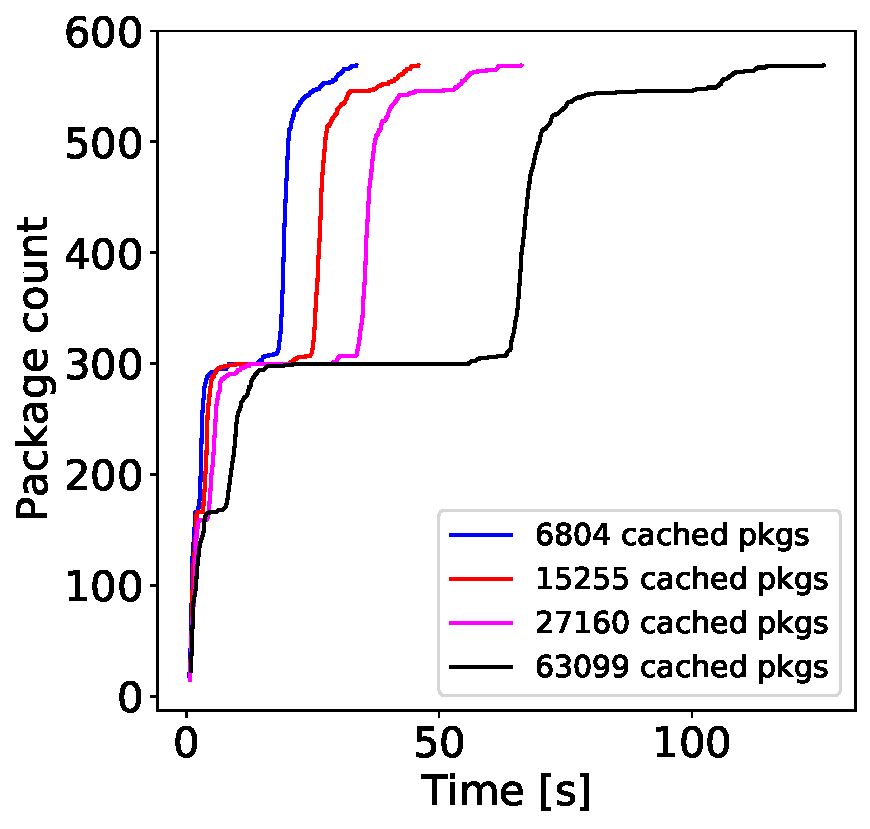
\includegraphics[width=0.32\textwidth]{figures/perf/cdf_e4s_cache_lassen_total_fig.pdf}
    }
    \caption{Cumulative distribution of solve times for different cache sizes across all E4S packages on the Lassen machine.}
    \label{fig:cdf_e4s_lassen}

\end{figure*}


We specifically focus on the packages in the ECP Extreme-scale Scientific Software Stack
(E4S) project~\cite{e4s}. It is a community effort to provide open source software
packages for developing, deploying, and running scientific applications on HPC
platforms. There are just under 600 packages in E4S, but the buildcache of the project
targets different architectures, operating systems, and compilers, thereby totaling over
60K pre-compiled packages (hash signatures). We divided the buildcache into 4 groups:
full buildcache (63099 packages), buildcache restricted to the \texttt{ppc64le}
architecture (27160 packages), buildcache restricted to the \texttt{rhel7} OS (15255
packages), and buildcache restricted to both \texttt{ppc64le} architecture and the
\texttt{rhel7} OS (6804 packages). Benchmarking across an increasing size of the
buildcache provides us with a better understanding of the impact of reuse optimization.


Figures~\ref{subfig:cdf_e4s_quartz_load_a}, \ref{subfig:cdf_e4s_quartz_solve_a},
and~\ref{subfig:cdf_e4s_quartz_full_a} show the cumulative distribution of the solve
times of the E4S packages with increasing buildcache on Quartz. The results on Lassen
are comparable to Quartz and are omitted to save space. Setup times are higher than
solve times, even for smaller buildcaches. This happens because when we reuse packages
we need to load the database of existing packages. This is currently time consuming
because it requires us to read and compare many spec objects in Python. There a jump in
the solve times for the largest buildcache, but most solves take less than 10 seconds.
The fact that the runtime is dominated by serial setup time is good news; setup time is
easily optimized away through caching and optimizing Python code, while solve
time is not. The E4S buildcache, with nearly 64,000 packages, is much larger than most
package repositories, and we expect that our approach will scale to much larger
buildcaches if we can optimize the Python runtime. Multi-shot solver techniques may
offer additional solver performance, as we can divide and conquer for a slightly less
optimal final result.

% 
\begin{figure*}[htb]

    \centering
    \subfloat[][Ground times vs. number of dependencies]{
    \label{subfig:deps_quartz_load_a}
        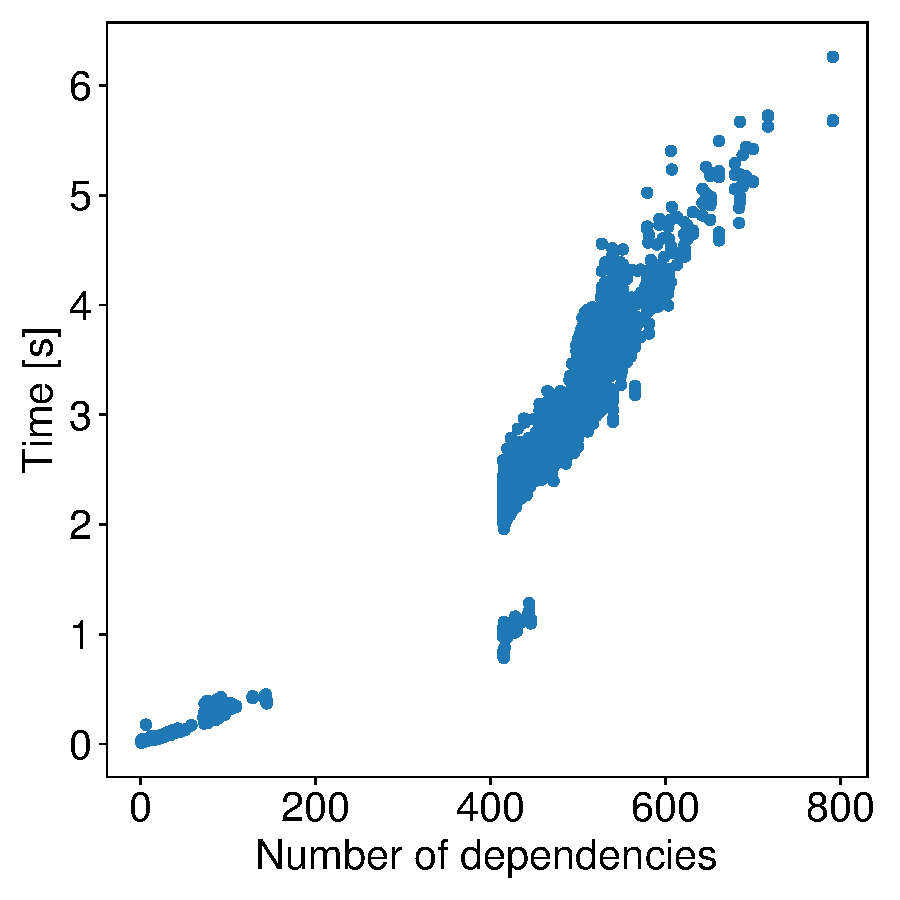
\includegraphics[width=\perfsubfigwidth\textwidth]{figures/new-quartz/deps_quartz_ground_fig.pdf}
    }\hfill%
    \subfloat[][Solve times vs. number of dependencies]{
    \label{subfig:deps_quartz_solve_a}
        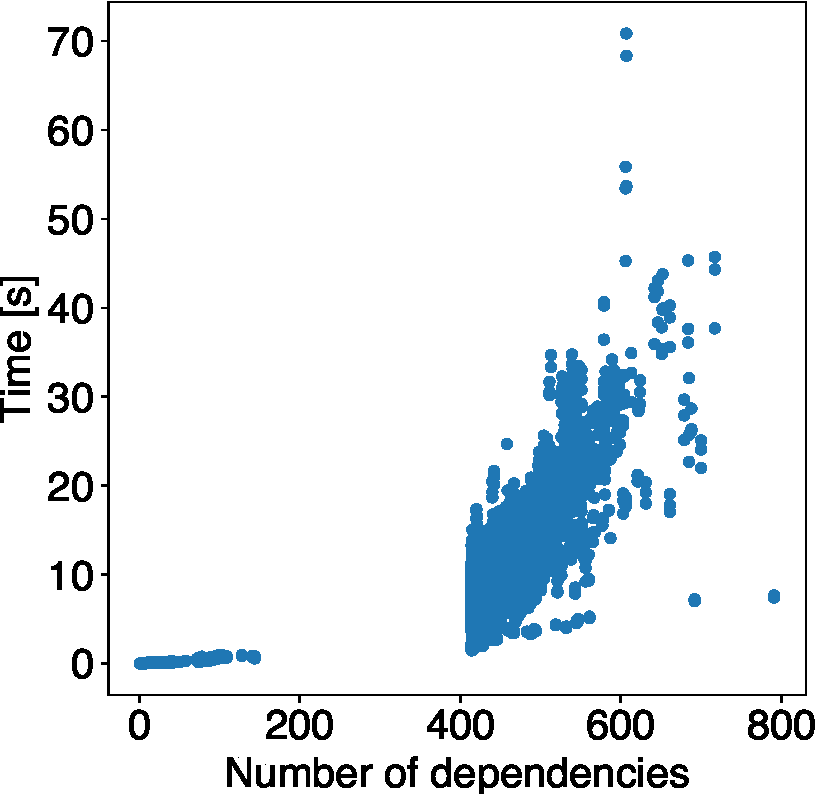
\includegraphics[width=\perfsubfigwidth\textwidth]{figures/new-quartz/deps_quartz_solve_fig.pdf}
    }\hfill%
    \subfloat[][Full solving times vs. number of dependencies]{
    \label{subfig:deps_quartz_full_a}
        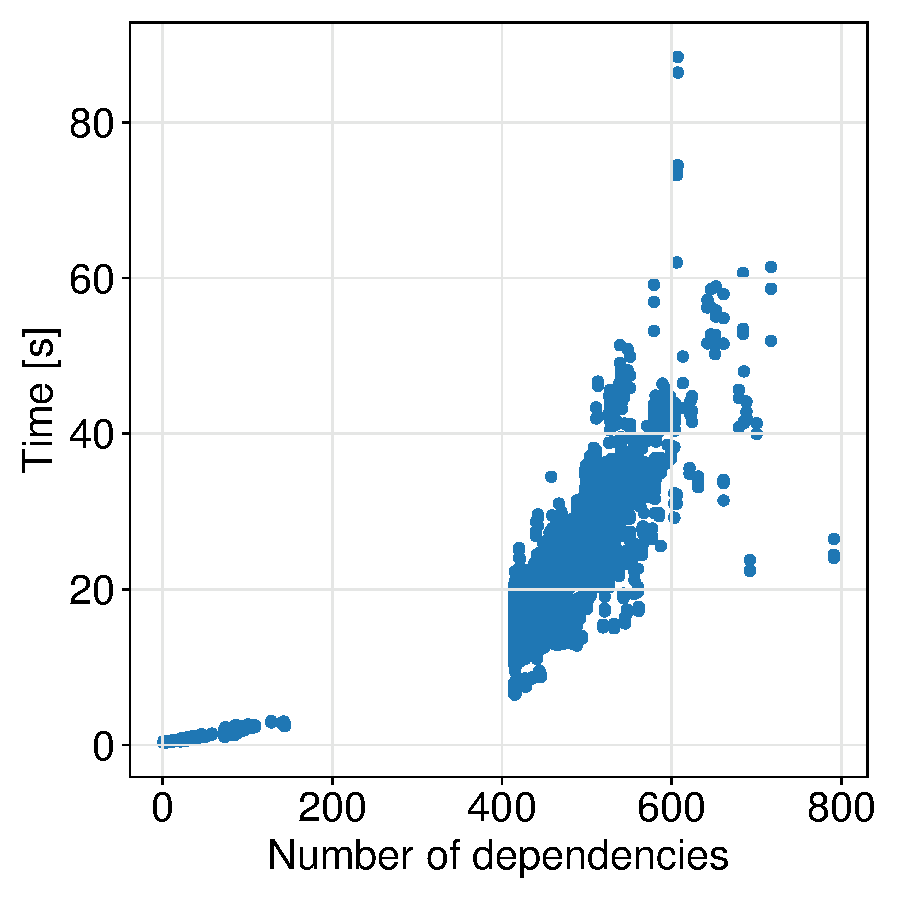
\includegraphics[width=\perfsubfigwidth\textwidth]{figures/new-quartz/deps_quartz_total_fig.pdf}
    }\hfill%
    \subfloat[][CDF of full solving times under various configurations]{
    \label{subfig:cdf_quartz_full_a}
        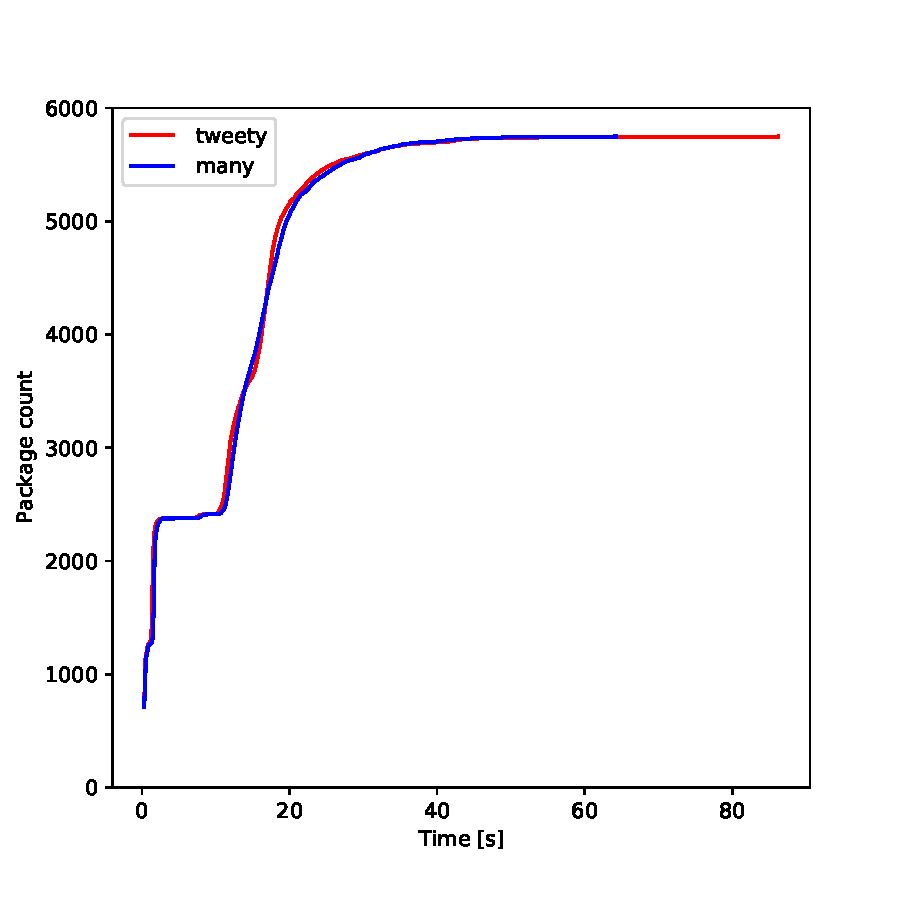
\includegraphics[width=\perfsubfigwidth\textwidth]{figures/perf/cdf_quartz_total_fig.pdf}
    }\\
    \subfloat[][CDF of setup times for different cache sizes across all E4S packages]{
    \label{subfig:cdf_e4s_quartz_load_a}
        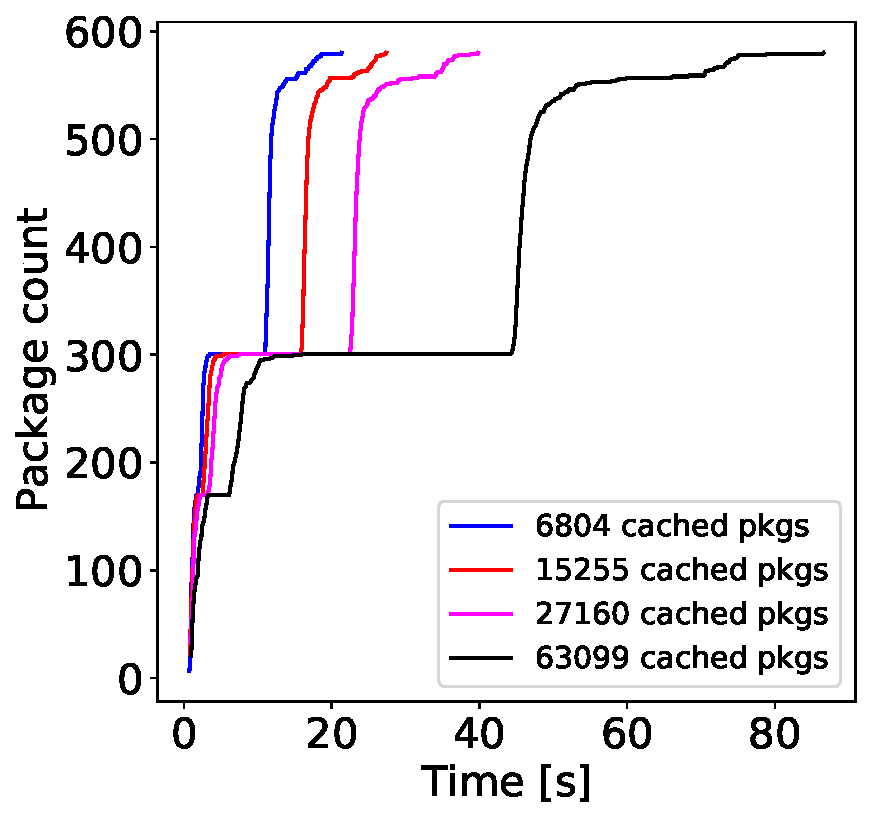
\includegraphics[width=\perfsubfigwidth\textwidth]{figures/perf/cdf_e4s_cache_quartz_setup_fig.pdf}
    }\hfill%
    \subfloat[][CDF of solve times for different cache sizes across all E4S packages]{
    \label{subfig:cdf_e4s_quartz_solve_a}
        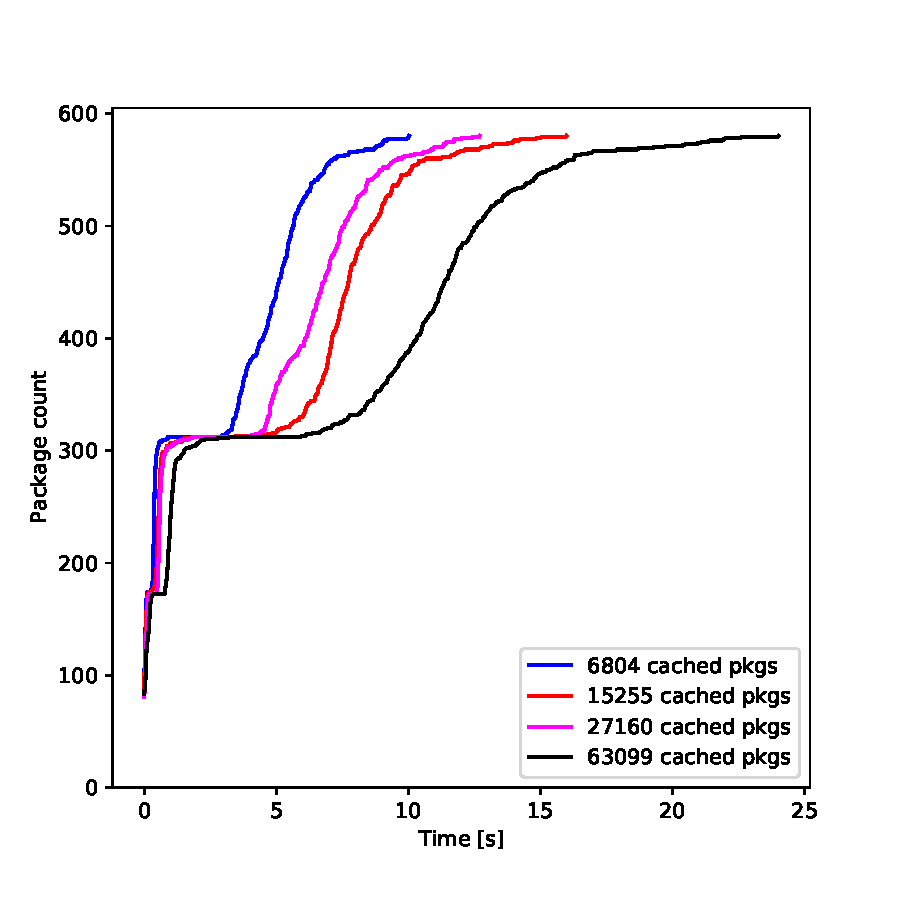
\includegraphics[width=\perfsubfigwidth\textwidth]{figures/perf/cdf_e4s_cache_quartz_solve_fig.pdf}
    }\hfill%
    \subfloat[][CDF of total solver times for different cache sizes across all E4S packages]{
    \label{subfig:cdf_e4s_quartz_full_a}
        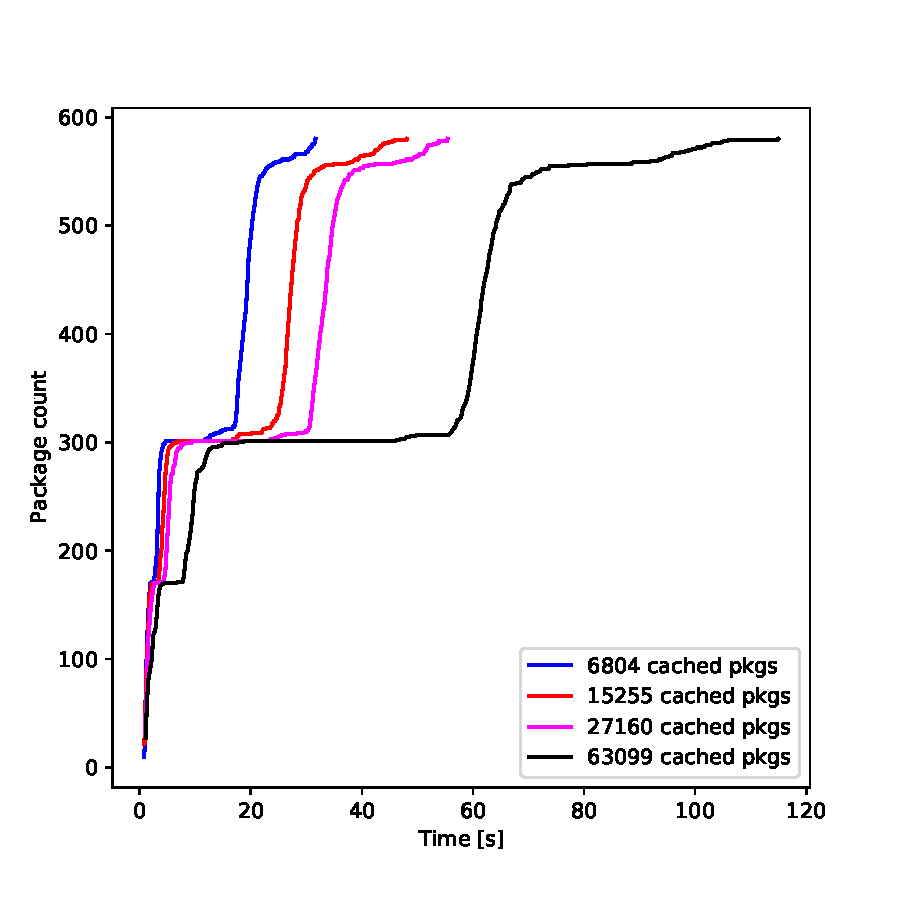
\includegraphics[width=\perfsubfigwidth\textwidth]{figures/perf/cdf_e4s_cache_quartz_total_fig.pdf}
    }\hfill%
    \subfloat[][CDF of old concretizer concretization times and \clingo{} total solve times]{
    \label{subfig:cdf_old_vs_new_a}
        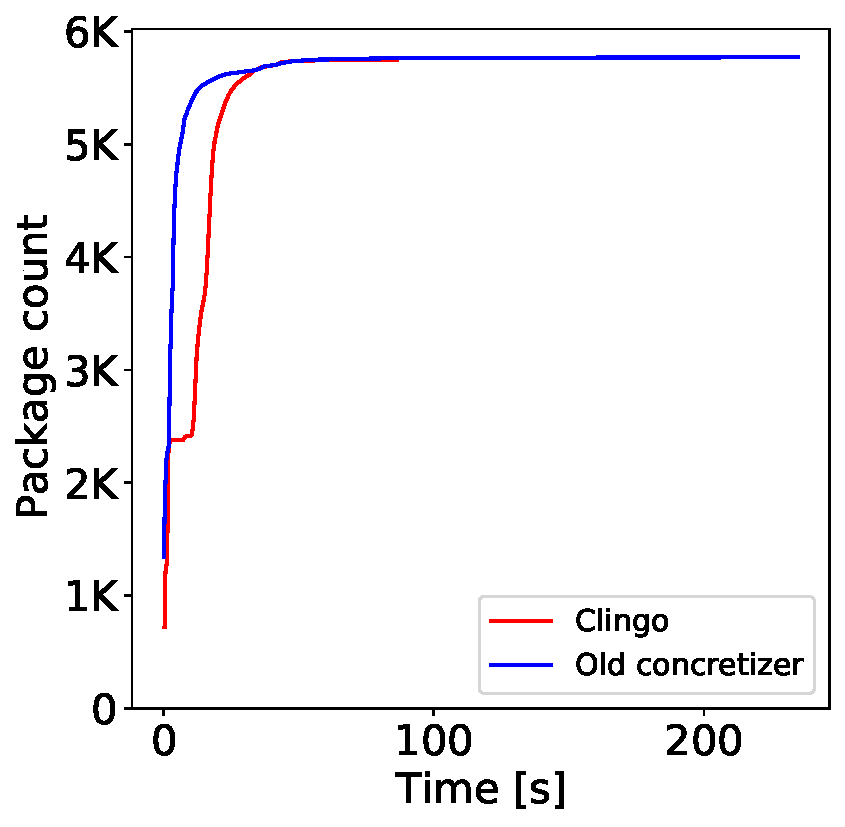
\includegraphics[width=\perfsubfigwidth\textwidth]{figures/perf/cdf_quartz_old_vs_clingo.pdf}
    }

    \caption{Performance figures of solving times across all packages on Quartz.\vspace{-1em}}
    \label{fig:all_perf}

\end{figure*}

